\documentclass[UTF8]{ctexart}
\usepackage{graphicx}
\usepackage{float}
\usepackage{subfigure}
\usepackage{geometry}
\usepackage{fancyhdr}
\usepackage{lastpage}
\usepackage{color}
\usepackage{framed}
\usepackage{fontspec}
\usepackage{cite}

\geometry{left=2.54cm,right=2.54cm,top=3.18cm,bottom=3.18cm}
\definecolor{shadecolor}{rgb}{0.95,0.95,0.95}
\pagestyle{fancy}
\lhead{
\includegraphics[scale=1]{sjtu-logo-red.pdf}}  
\rhead{肱骨干骨折术后康复器} 
\cfoot{第 \thepage\ 页\ 共 \pageref{LastPage} 页} 

\begin{document}

\begin{titlepage}
    \begin{center}
        
\includegraphics[width=0.8\textwidth]{sjtu-name-blue.pdf}\\[1cm]
        \textsc{\huge \bfseries 课程项目报告}\\[1.5cm]
        
\includegraphics[width=0.3\textwidth]{sjtu-badge-blue.pdf}\\[1cm]    
        \textsc{\huge \bfseries 生物医学工程导论作业三}\\[1.5cm]


        \Huge \bfseries{肱骨干骨折术后康复器}\\[1cm]
            
        \Large \bfseries{裴奕博518021910971\\许世杰518021910257\\李启隆518082910008\\王文才518021910585\\}

    \end{center}
\end{titlepage}


\section{摘要}
    本课程项目的产品名称为:肱骨干骨折术后肘关节矫正器。

    近年来,随着人口老龄化的加剧和意外事故发生率的上升,骨折病人的数量正处在逐年增加之中。对于一个骨折病人来说,骨折部位附近在经历一段时间的外固定(石膏、夹板固定)或者内固定(如手术后钢板、钢钉固定),后,会出现关节僵硬、肌肉萎缩等并发症。因此骨折病人在接受治疗后,需要经过一段漫长的康复时间。而这些骨折绝大多数是位于四肢的骨折,康复起来比较困难。因此我们从这一实际需求出发,针对其中肱骨骨干骨折的病人,设计了康复矫正器,运用电、热、机械等多种物理方式,辅助病人进行康复。在设计过程中,我们充分利用现有的技术手段,并对其加以整合,可行性较强。我们相信,我们的产品在获得临床数据支持后,投入实用较为容易。此外,对于其他部位的矫正器械,我们也提出了相应的推广方法和一些展望,使得我们设计的医疗器械能够适应更多的病人和状况。
\newpage
\section{项目背景}
    \subsection{项目需求}
        随着人口老龄化的加剧和以外事故发生率的逐年上升,骨折的发病率和骨折病人的数量都在逐年上升。目前,全球正在经历着人类历史上最巨大的人口结构变化,随着人均寿命延长,全球进入了人口高速老龄化时期。我国也不例外,2013年,60岁以上人口约占人口总数的15\%;预计至2050年,60岁以上人口将达到我国总人口的25\%。“长寿奇迹”所带来的直接后果将是困扰老年人的疾病的爆发,首当其冲的就是骨质疏松、跌倒以及随之而来的脆性骨折。
        
        数据显示中国患骨质疏松症已跃居常见病多发病的第七位,中国内地总患病率为12.4\%,老年人中患病比例超过一半以上,其中骨折发生率接近1/3,这已经是一个相当可怕的数字。来自英国南安普敦大学和谢菲尔德医学院的一项研究表明,在未来三十年内,脆性骨折的负担将会急剧增加。到2040年,骨折高风险人群数量大约为3.19亿——这个数字比今天的高风险人群数量增加一倍。
        
        肱骨干骨折占全身骨折的3~5\%,属于常见骨折部位。肱骨干骨折常见于成年人,易受骨质疏松影响。如今肱骨干骨折的治疗手段已经趋于完善,根据骨折的严重程度,无论是保守疗法(悬吊石膏或功能支具固定)还是手术治疗(多种内固定术,包括微创手术)\cite{Ref1}都已经非常成熟。然而,相比治疗,骨折病人的康复训练更应受到我们的关注。
        
        骨折病人为什么需要康复训练呢?原因主要在于康复训练不及时所导致的种种并发症。这些并发症归根到底可分为两类:

        \begin{enumerate}
            \item[\textbf{1)}]关节问题
            
                这是骨折患者最常见的并发症, 主要是因为石膏的长期固定, 关节没有得到活动, 局部血流速度变慢, 纤维蛋白渗出后在局部积聚等多种原因, 引起部分组织发生黏连, 导致关节僵硬现象, 对患者的生活与工作造成影响。特别的,对于本项目需要研究的肱骨干骨折患者,由于长时间采用图\ref{Fig.sub.1}方式固定,长时间保持一种姿势,若不及时进行康复训练可能会造成如图\ref{Fig.sub.2}肘关节僵硬而无法伸直的情况。
                \begin{figure}[H]
                    \centering  %图片全局居中
                    \subfigure[肱骨干骨折固定图]{
                    \label{Fig.sub.1}
                    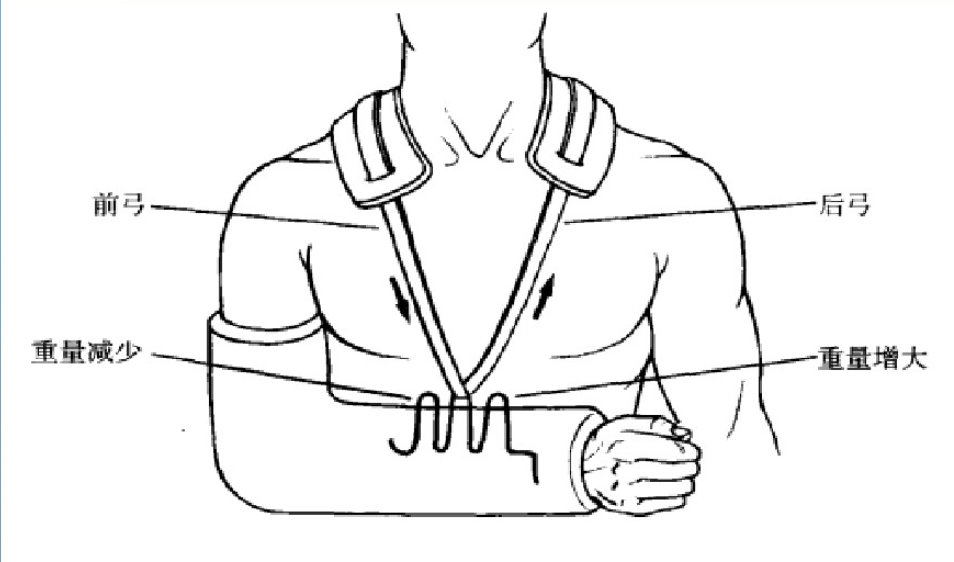
\includegraphics[width=0.5\textwidth]{fixed1.png}}
                    \subfigure[关节僵硬症状]{
                    \label{Fig.sub.2}
                    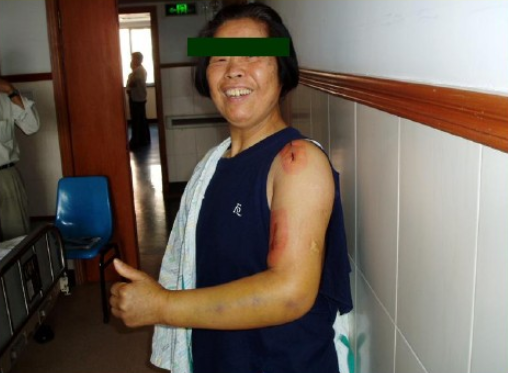
\includegraphics[width=0.4\textwidth]{fixed2.png}}
                    \label{Fig.main}
                    \caption{关节问题}
                \end{figure}
                    
            \item[\textbf{2)}] 肌肉问题
             
                另外一种容易出现的并发症是是肌肉无力和萎缩问题:患肢的骨骼肌因得不到足够的力学刺激,新陈代谢大大降低,出现废用性萎缩,而骨骼肌的萎缩又限制了关节用肢体功能的恢复。\cite{Ref2} 
        \end{enumerate}

        为解决肱骨干骨折病人的康复训练问题,特提出本项目构思,即我们希望可以有一个器械可以在骨伤恢复的同时即进行针对于这种由于长期固定带来的肌肉及关节问题进行康复。
    \subsection{肱骨干骨折病人的康复现状及存在的问题}
        \subsubsection{康复现状}
            目前,肱骨干骨折病人的主要康复措施主要是病人自身的功能锻炼,还有其他的光疗、蜡疗等效果并不显著的“非正常”疗法。

            关于功能锻炼,在此给出一个标准的肱骨干骨折术后康复疗程:
            \begin{shaded}
                \textsl{
                    2~3周,站立位,主动耸肩练习10~20次,肩关节放松自然下垂,10次为1组,持续30秒;做胸大肌、背阔肌群收缩练习;三角肌保护性的无阻力收缩练习,持续时间及次数由治疗师自行掌握,以无疼痛为限。肩部的摆动次数练习,10次1组,做2~3组为宜;增加前臂的内外旋度练习,10次1组,做2~3组;肘关节做屈伸功能练习,主动收缩为主,不增加阻力,以患者感觉疲劳为限。}
                
                    \textsl{4~6周,在上述基础上,增加肩、肘、腕的抗阻力练习,加强前臂的内外旋功能训练。}
                
                    \textsl{6~8周,患侧上肢自然,以肩关节为轴心,做主动全旋练习,借助肋木,滑轮、墙拉力器,橡皮带等器械进行功能练习。}
            \end{shaded}
        \subsubsection{存在的问题}
            从上面的康复流程我们可以看到,肱骨干骨折术后的康复过程是一个漫长而又艰辛的过程。在这漫长的过程中,存在着以下几点缺陷:
            \begin{enumerate}
                \item [\textbf{1)}]康复时间过长 
                
                    六到八周的康复时间过长。通常情况下,患者会在第三周左右骨伤基本复原并开始恢复自己的学习或工作,而这种康复问题基本依赖患者的自觉。康复时间过长对于患者的生活水平也会造成不小的影响
                
                \item [\textbf{2)}]康复效果不佳
                    
                    康复的早期应该是规避并发症的最佳时机。但由于手术固定的石膏、一开始疼痛感强等锻炼力度往往较小,缺乏辅助设备来帮助进行更高强度的锻炼。这也导致大部分病人在6~8周的康复期过后仍然达不到期望的康复效果。

                \item [\textbf{3)}]缺乏有效指导
                
                    康复的整个过程基本都在家中进行,整个过程缺乏护理医师的指导。患者很难通过自身的反应来实时调整自己的康复计划。
            
                \item [\textbf{4)}]传统观念的影响
                
                    现在的许多患者仍然被传统观念束缚且对传统观念中“伤筋动骨一百天”的认识有所误解。比如有些患者会认为在这100天内不应该 去触碰受伤部位,更别提康复了。这导致部分患者对于这种康复问题的重视度特别低。
            \end{enumerate}

    \subsection{项目的目的和意义}
        经过以上背景的分析,本项目的目的和意义如下:
            \begin{enumerate}
                \item [\textbf{1)}]为肱骨干骨折的患者提供一种能帮助他们缩短康复疗程、提升康复效果的康复器械,尽可能减少患者在康复期间因为行动不便而对生活造成的影响。
                \item [\textbf{2)}]创新康复的方式。通过多种手段结合而不是简单的模拟康复训练的方式以提升康复效果。
                \item [\textbf{3)}]让病人在家中也能使用辅助器械进行康复,而不是一想到康复就只能去医院。
            \end{enumerate}
\newpage
\section{项目方案设计}
    \subsection{整体结构设计}
        在整体结构的设计上,我们首先有如下几点考虑:
        \begin{enumerate}
            \item[\textbf{1)}]使用场景的限制
            
            由于项目的使用场景主要是家用,因此体积不应该过大,最好做成便携式以适应更广泛的应用场景。
            \item[\textbf{2)}]康复方式的选择
            
            根据现有的较成熟的技术和市面上已有的产品考虑,并针对上文所述的容易出现的两类并发症。我们最终采用以机械牵拉为主、电刺激和加热为辅的方式,而放弃了磁疗、蜡疗等具体作用机理还不清楚的康复方式。通过多种物理方式的协同工作以提升康复效果。
            
            \item[\textbf{3)}]用户操作的便利性
                我们希望我们的装置能够做到统一供电、统一控制、统一操作。这样可以降低患者的学习成本,使得装置更易用。 
        \end{enumerate}
        在以上几点原则的基础上,我们最后提出的设计方案图如下:
        \begin{figure}[H]
            \centering
            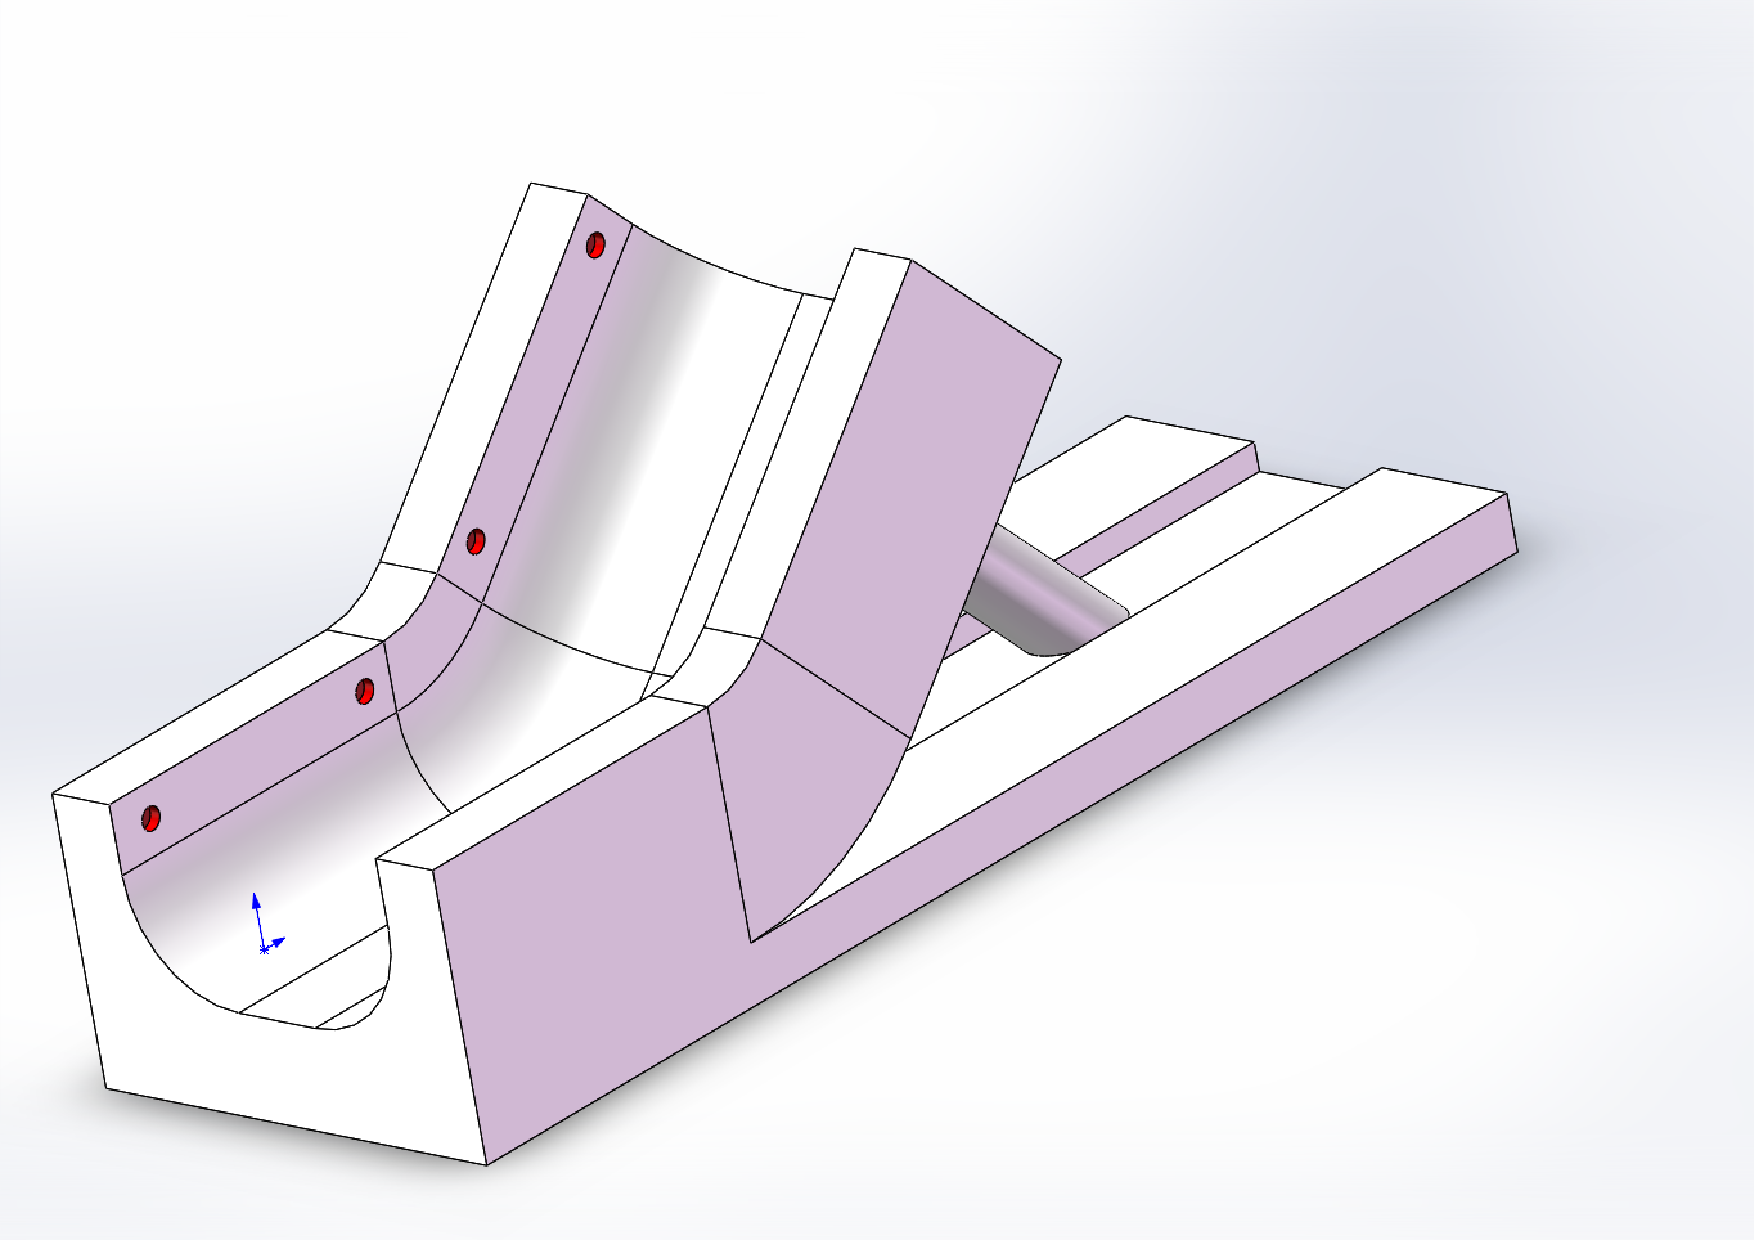
\includegraphics[width=0.7\textwidth]{General_Design.pdf}
            \caption{总体方案示意图}
            \label{General}
        \end{figure}
        \begin{figure}[H]
            \centering
            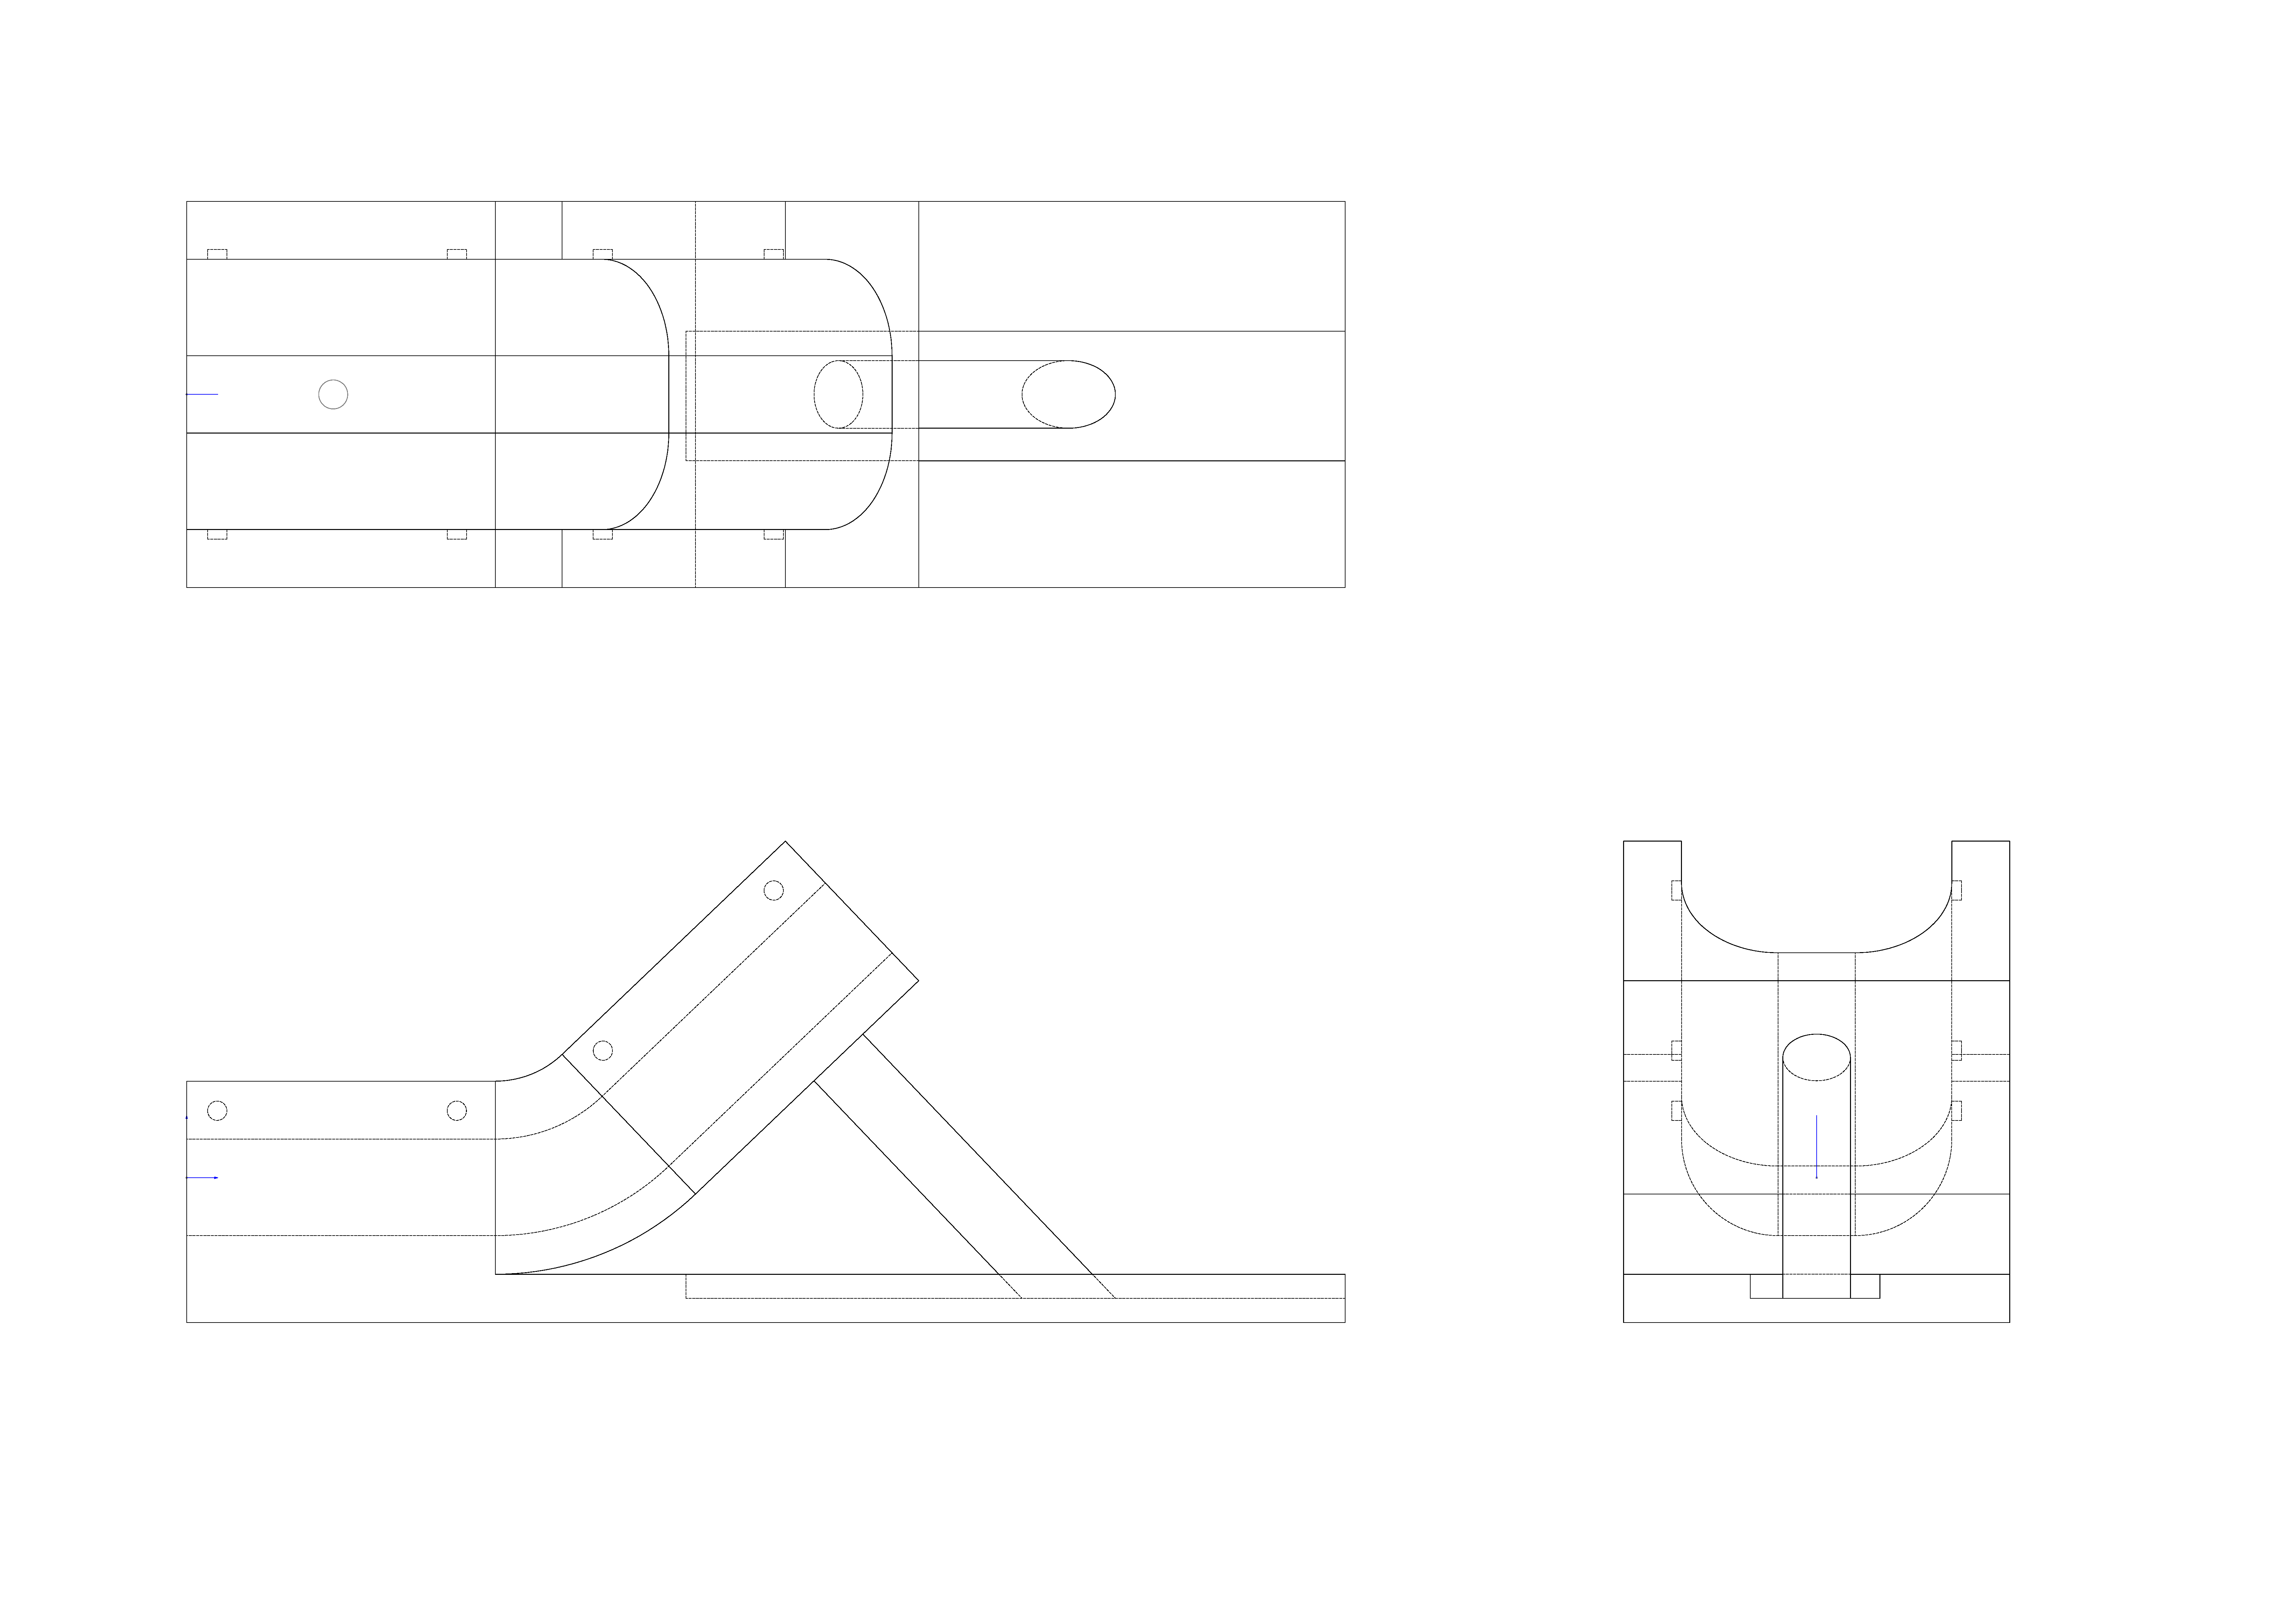
\includegraphics[width=0.7\textwidth]{3D_Figure.pdf}
            \caption{方案三视图}
        \end{figure}
        项目主体由三部分组成:一个U形槽、一条滑轨和一根支撑柱组成。下面分别简述三部分的结构和功能:
        \begin{enumerate}
            \item[\textbf{1)}]U形槽

                U形槽分为两段:一段与滑轨合为一体,通过一个转轴与另一段U形槽相连。所有的供能装置、加热装置和电刺激装置均整合在U形槽内。U形槽的主要功能是放置患肢和对患肢进行固定。在U形槽的外侧还有四组绑带(图中未画出),防止患者的肢体在机械牵拉过程中从U形槽中脱出。

            \item[\textbf{2)}]滑轨

                滑轨被放置在整个装置的底部,使用时与桌面贴合,主要用于传动。其主要功能是使得支撑柱在其中滑动,改变两段U形槽之间的角度以达到牵拉目的。
            \item[\textbf{3)}]支撑柱  

                支撑柱是U形槽和滑轨之间的连接。支撑柱不可伸缩,与U形槽通过转轴连接,与滑轨形成可滑动的连接。
        \end{enumerate}
        
    \subsection{各部分细节设计}
        \subsubsection{热刺激装置设计}
            针对患者关节处因长期无法活动而造成的代谢问题,我们设计热刺激装置以增强关节处局部的新陈代谢,起到活血化瘀的功能,防止纤维蛋白沉积使得关节僵硬。

            热刺激装置全部集成于U形槽内,主要由温控装置和加热装置组成。温控装置可以实时监控当前温度,使当温度达到使用者设定的指定温度时自动停止加热,温度降低后加热继续,以维持温度的稳定。加热装置沿着U形槽轮廓排布,使用电热丝加热,与其他用电装置通过统一的电源供电。
        \subsubsection{机械结构设计}
            针对患者关节处产生的关节僵硬的并发症,我们设计机械牵拉装置,用最直接的方式解决这一问题。我们希望可以通过机械装置周期性牵拉,使得手臂肌肉受到周期性的收缩和舒张,同时环节关节处的僵硬情况。
            \begin{figure}[H]
                \centering
                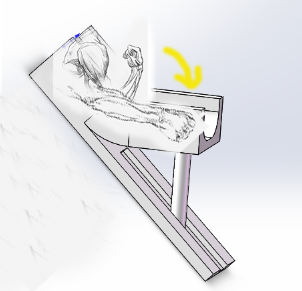
\includegraphics[width=0.5\textwidth]{Machine.png}
                \caption{机械装置示意图}
                \label{fig:Machine}
            \end{figure}

            机械结构的动力装置与其他装置的动力一样,置于U形槽底部,采用电机驱动。两端U型槽通过转轴连接,通过转轴旋转可实现手臂的屈伸动作。如图\ref{fig:Machine},传动装置(示意图中未画出)位于滑轨中,我们从千斤顶中获得灵感,采用螺杆传动的方式。通过螺杆的转动带动支撑柱下端在滑轨上周期性移动,从而带动转轴旋转实现牵拉功能。螺杆的活动范围和电机的转速均可调,这两个参数也对应了牵拉的角度范围和牵拉的速度。
        \subsubsection{电刺激结构设计}
            针对患者出现的肌肉萎缩和废用性退化的问题,我们设计了电刺激装置,其灵感来源于已经在运动员训练中被广泛使用,不久前进入健身领域的肌肉电刺激$(Electrical Muscle Stimulation,EMS)$技术。\cite{wiki}

            \begin{figure}[H]
                \centering  %图片全局居中
                \subfigure[EMS原理]{
                \label{fig:EMS_Principle}
                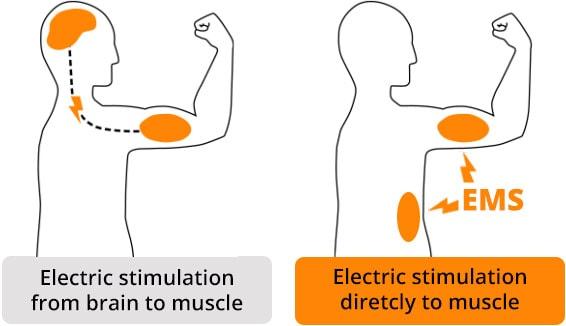
\includegraphics[width=0.5\textwidth]{core-technology-ems.jpg}}
                \subfigure[EMS使用]{
                \label{EMS}
                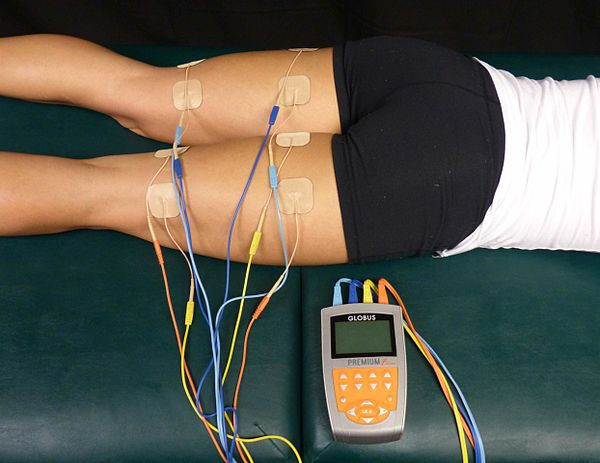
\includegraphics[width=0.4\textwidth]{ems.jpeg}}
                \label{Fig.main}
                \caption{EMS原理及使用}
            \end{figure}
           
            如图\ref{fig:EMS_Principle},该技术的原理非常简单:正常人的肌肉活动过程是由大脑发出动作电位,一路传播到特定的肌肉部位,刺激相应的肌肉收缩。EMS的原理就是将大脑发出的信号直接用外界的电刺激代替,即不经过大脑,直接刺激对应的肌肉。如图\ref{EMS}使用时将电极贴在肌肉的两端即可达到此目的。数据显示,使用EMS技术进行日常训练的运动员的肌肉力量最多可以在正常训练的基础上增强约40\%。

            我们将这一技术集成在我们的装置中。根据手臂肌群的位置(肱二头肌、肱三头肌均位于左右两侧),我们将4组电极嵌入U形槽侧面(见图\ref{General}中标红色的凹槽位置),分别置于大臂、前臂肌群的两端。使用时只需使手臂贴紧U形槽侧面,该装置即可发挥作用。电刺激的强度可以根据需要调节,确保刺激强度具有锻炼效果而又不会使得肌肉僵直。
    \subsection{项目特点}
        通过以上设计,我们提出的项目方案具有如下几个特点:
        \begin{enumerate}
            \item[\textbf{1)}]体积小
             
                相比医院中的立式、柜式康复系统,本项目方案体积较小,总长度不超过$1m$,更适合家用。
            \item[\textbf{2)}] 功能完善
            
                通过热刺激装置、机械装置和电刺激装置的整合,我们基本实现了当初的设想,即采用多种康复手段结合的方式辅助患者康复。 
            \item[\textbf{3)}]集成化程度高
                
                所有装置做到统一供能、统一控制。且所有装置均集成在U形槽内,集成化程度较高。
        \end{enumerate}
\newpage

\section{项目不足与展望}
    \subsection{项目不足}
        总体来说,我们的项目其实已经比较完善,技术条件已经基本成熟,实现起来也比较方便,但仍然存在以下几点不足:
        \begin{enumerate}
            \item [\textbf{1)}]项目适用性不足。
            
            我们的项目设计针对的是是肱骨干骨折,由于骨折部位离关节较远,相对来说固定和康复比较容易。同理,对于股骨、胫腓骨、尺桡骨等长骨的骨干骨折,我们仍然可以用类似的方法解决。但是如果患者骨折的部位位于关节处,由于关节处更加复杂,也相对比较灵活,一般情况下的处理方式都是进行石膏全包装并且无法活动。因此这种情况下,机械牵拉的方式很难继续实行。如果强行进行机械牵拉康复,很可能会造成骨折处的移位等再次伤害。在这一点上,我们的方式适用性不够。然而实际上,在日常生活中,长骨中段骨折所占的比例并不是多数,对于最常见的桡骨远端、胫腓骨远端的骨折,均可能因为骨折部位靠近腕关节和踝关节,康复效果有限。因此在康复部位的适用性上,我们的项目还有局限。

            \item [\textbf{2)}]治疗手段有限
            
            我们的治疗手段还比较有限,目前设计想法主要是将加热治疗,机械牵引还有电刺激相结合实行康复治疗。这些是相对比较成熟一些的技术。但是考虑的整个康复过程的持续性,我们更希望还有一些新的治疗手段的加入。比如当前有资料显示,磁场对人身体有一定的治疗能力已经被证实,但具体如何治疗并没有定论,我们的设计还未能加入这样的方式。

            \item [\textbf{3)}]缺乏临床数据支持
            
            我们的设计主要通过物理手段来实现康复过程,因此其中一些物理参数的设定对于康复的有效性、效果和安全性起着十分关键的作用。比如机械部分的牵拉角度能够产生恢复效果而不会因为过度牵拉对机体造成伤害。此外,机械装置的牵拉速度,电刺激装置的刺激强度等参数也有类似的问题。要解决这一问题,需要实验和临床数据的支持。而这一点是我们当前的设计还缺乏的。
        \end{enumerate}
    \subsection{项目展望}
        根据我们项目本身的特点和不足,我们小组在最后提出以下几点展望:
        \begin{enumerate}
            \item[\textbf{1)}]使用部位的推广
    
                我们希望我们的装置能在使用部位上有所推广,以便更加适用于更常见和更广泛的的骨折部位。从装置本身的设计来看,加热装置和电刺激装置比较容易推广,而机械牵拉装置是否能够在其他部位通用,需要进一步的探究。
            

            \item[\textbf{2)}]康复器械便携化
                我们设计这一装置时,当前的使用场景是家庭。但是我们最终的希望是整个装置能够做到便携化。这需要很高的集成化程度带来的体积的缩小。这一方面的工作也需要进一步开展。 

            \item[\textbf{3)}]治疗方式多样化
            
            本项目采用了机械牵拉、热刺激和电刺激三种方式协同作用。但是,在骨折患者的康复方面,还有其他方式可供我们选择。比如我们查阅相关磁场在医学上的功能发现,磁场能够促进成骨细胞生长,促进骨胶原蛋白的合成,抑制成脂细胞从而抑制骨腔中脂肪的增加。可以看到对于骨折后正常功能的恢复有相当好的效果。我们希望在这方面能够有更多样化的选择。
            

            \item[\textbf{4)}]加入有效的提醒方式
                
                针对康复周期过长,病人难以仅靠自觉维持康复训练的问题,可以设计相关的提醒装置。这一装置实现起来难度不高,但如何取得更好的效果需要进一步讨论。
            
            \item[\textbf{5)}]个性化参数制定
                
                由于不同的病人存在个体差异,我们希望可以制作一套科学的完整的康复流程和参数表。针对不同病人的不同康复阶段个性化地确定康复方案和相关参数。而这一设想还需要大量的临床数据支持和实验。
        \end{enumerate}

\bibliographystyle{plain}
\bibliography{Ref}
    
\end{document}
